\documentclass[a5paper,12pt]{book}
\usepackage{notes}
\begin{document}
\input{./tex/title.tex}
\clearpage
\tableofcontents
%\listoftables
\listoffigures
\clearpage

\chapter{Central forces}
%Derive angular momentum and total energy as constants of the motion
\clearpage

\chapter{Gravity}
%Introduce the inverse square law for gravity and show the eccentricity vector is a constant of motion under gravity
\clearpage

\chapter{Geometry of an Ellipse}
\section{The String Construction of an Ellipse}

One method of drawing an ellipse is to take a string of fixed length pinned to the two focus points of the ellipse. We can use this method to derive the standard equations for an ellipse. We will first start by setting up the geometry.

\begin{figure}[h]
\centering
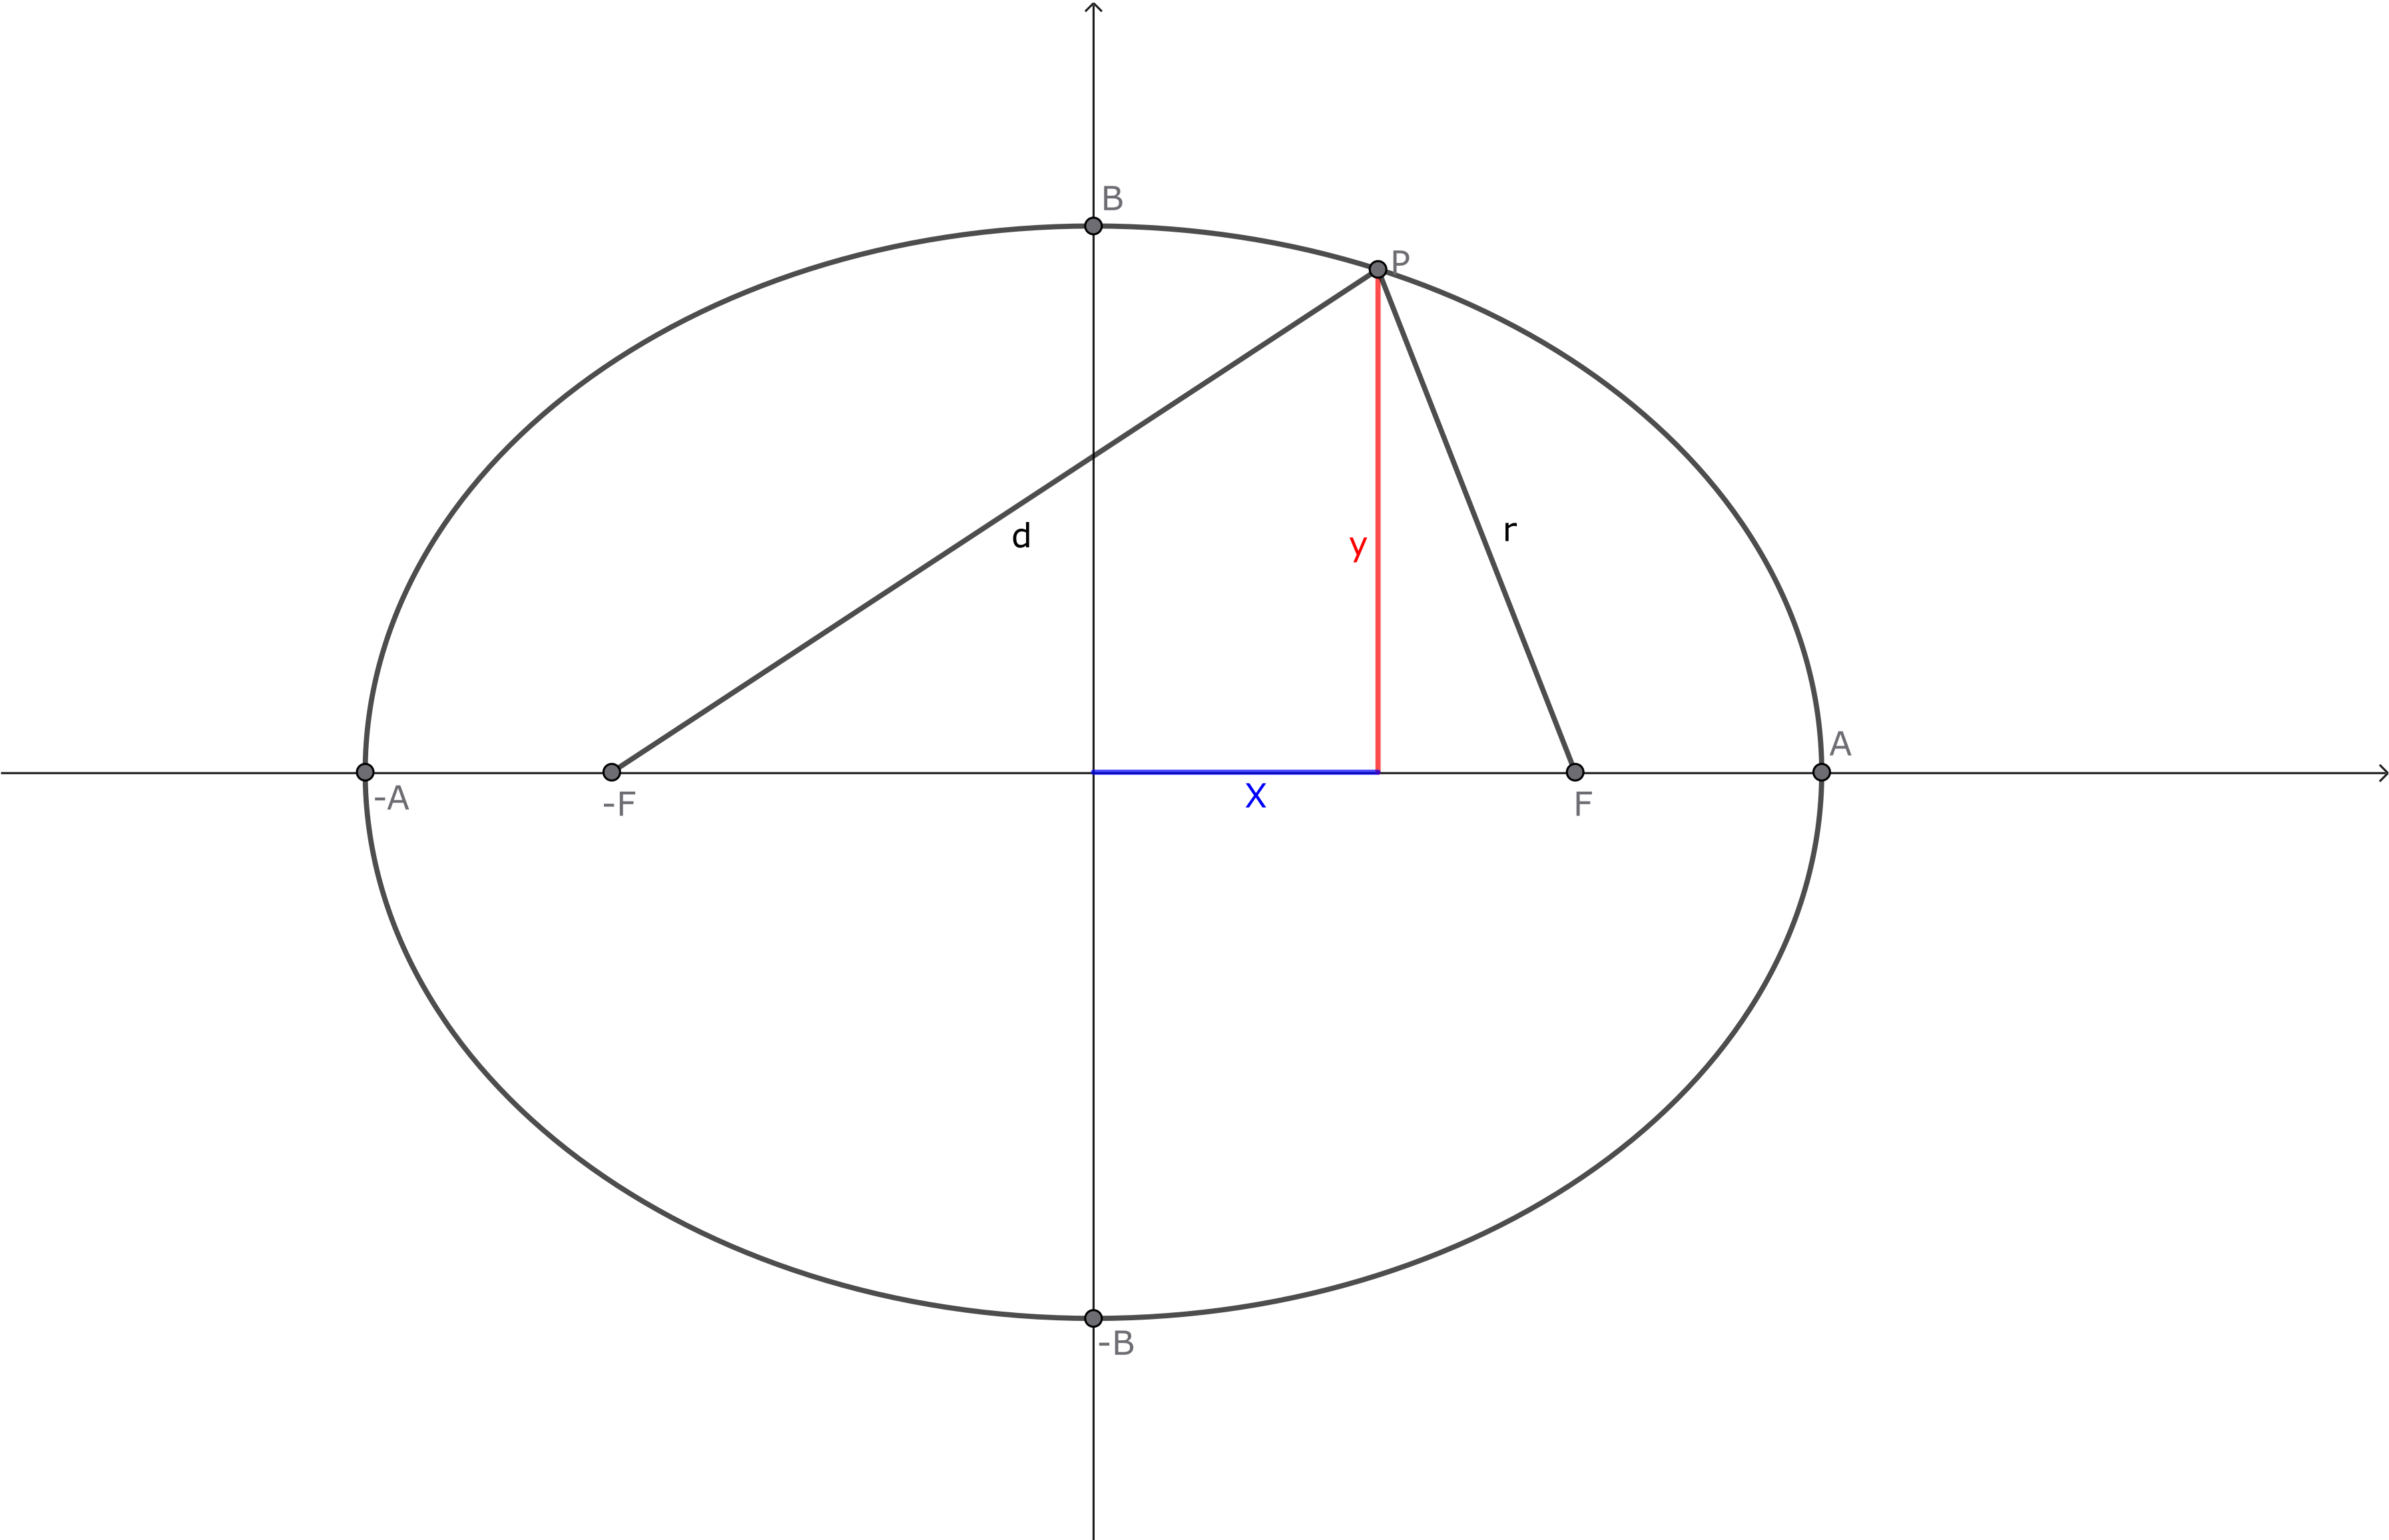
\includegraphics[height=0.3\textheight]{./img/string-method.png} 
\caption{The string method of constructing an ellipse} \label{fig:string-method}
\end{figure}

We will work in a two dimensional Cartesian coordinate system with an ellipse centered at the origin and orientated so that it's semi-major axis is directed along the x-axis and it's semi-minor axis orientated with the y axis. The two focus points $F$ and $-F$ are located on the x-axis a distance $f$ away from the origin, so that $F=(f,0)$ and $-F=(-f,0)$. Let $P$ be an arbitrary point on the ellipse with coordinates $P=(X,y)$\footnote{We use $X$ rather than $x$ here to avoid confusion with a later definition of $x$ as a distance measured from the focus $F$}.
The ellipse has semi-major axis length $A$ and semi-minor axis length $B$,  so that $-A \leq X \leq A$ and $-B \leq y \leq B$. Let $r$ be the distance from $F$ to $P$ and $d$ be the distance from $-F$ to $P$ and let the sum of these be S, so that

\begin{equation}
S = r + d
\end{equation}

where
\begin{align}
r &= \sqrt{(X-f)^2+y^2} \\ \nonumber
d &= \sqrt{(X+f)^2+y^2}
\end{align}

\subsection{Special cases and useful results}

From the construction method, we know that the sum is fixed.  We can find it's exact value by considering $P$ when $y=0$ and $X=A$, so that 
\begin{align}
r &= \sqrt{(A-f)^2+0^2}\\ \nonumber
&=  \sqrt{(A-f)^2}\\ \nonumber
&=  A-f\\ \nonumber
d &= \sqrt{(A+f)^2+0^2}\\ \nonumber
&= \sqrt{(A+f)^2}\\ \nonumber
&= A+f\\ \nonumber
S &= r + d \\ \nonumber
&= A - f + A + f\\ \nonumber
S &= 2A
\end{align}

This shows that the string must be twice the length of the semi-major axis to work.

Another interesting result is obtained when we look at the point $P=(0,B)$

\begin{align}
r &=  \sqrt{(0-f)^2+B^2}\\ \nonumber
&=  \sqrt{f^2+B^2}\\ \nonumber
d &= \sqrt{(0+f)^2+B^2}\\ \nonumber
&= \sqrt{(f^2+B^2)^2}\\ \nonumber
S &=2  \sqrt{(f^2+B^2)^2}
\end{align}

since we now know that $S=2A$ we can subtitute for $S$
\begin{align}
S &=2  \sqrt{(f^2+B^2)^2} \\ \nonumber
2A &=2  \sqrt{(f^2+B^2)^2} \\ \nonumber
A &=\sqrt{(f^2+B^2)^2} \\ \nonumber
A^2 &=f^2+B^2
\end{align}

You are more likely to see this stated as $B=A\sqrt{1-e^2}$ where $e$ or the eccentricity is defined to be 

\begin{equation}
e=\frac{f}{A} \label{eq:eccentricity}
\end{equation}

so that $f=eA$

\subsection{Equation of an ellipse}

Now we know the value of $S$ we can look for a general equation that links $X$ and $y$. Firstly we write out the sum in full

\begin{align}
S & = r + d \nonumber \\
&= \sqrt{(A-f)^2+y^2} +  \sqrt{(A+f)^2+y^2}
\end{align}
\clearpage

\chapter{Perifocal plane}
%Introduce the perifocal plane and the coordinates in that plane. Derive the angular momentum and total energy in these coordinates
\clearpage

\chapter{Elliptical Orbits}
%Show that the equations of motion in the perifocal coordinate system lead to elliptical orbits.
\clearpage

\chapter{Kepler's Equation}
%Derive Kepler's Equation to show time evolution in the perifocal plane
\clearpage

\chapter{Initial Conditions}
% note include determining the alignment of the perifocal coordinates in 3d space
\section{Specific Total Energy}
\section{Specific Angular Momentum}
\section{Eccentricity Vector}
\section{Direction of Perifocal Plane}
\section{Phase of the Orbit, $M_0$}
\section{Time evolution of the position}
\clearpage

\chapter{Old Stuff to review}

\section{Plane Polar Coordinate System}
\input{./tex/PlainPolar.tex}
\clearpage

\section{Gravity}\label{sec:Gravity}
\input{./tex/Gravity.tex}
\clearpage

\section{Angular Momentum}
The angular momentum of a particle is given by
\begin{align}
\bm{L}&=\bm{r} \times \bm{p} \nonumber \\
&=m \bm{r}\times \frac{d \bm{r}}{d t} \nonumber \\
&=m r \hat{\bm{r}} \times \left[ \dot{r} \hat{\bm{r}} + r \omega \hat{\bm{\theta}} \right] \nonumber \\
&=m \left[ r \dot{r}\hat{\bm{r}} \times \hat{\bm{r}} + r^2 \omega \hat{\bm{r}} \times\hat{\bm{\theta}} \right] \nonumber \\
&=m r^2 \omega \uveck \label{eq:AngularMomentum}
\end{align}

We can also write this as $\mathbf{L} = l \uveck$ were
\begin{equation}
l=mr^2\omega \label{eq:AngularMomentumScalar}
\end{equation}

\subsection{Conservation Of Angular Momentum}
We can show now that angular momentum is conserved under a central force by taking the derivative with respect to time.

\begin{equation}
\frac{d\mathbf{L}}{dt} = \frac{d l \uveck}{dt} = \frac{d l}{dt}\uveck
\end{equation}
\begin{align}
\frac{dl}{dt}&=m\frac{d}{dt}\left[r^2\omega\right]\nonumber \\
&=m\left[\frac{dr^2}{dt}\omega + r^2\frac{d\omega}{dt}\right]\nonumber \\
&=m\left[\frac{dr^2}{dr}\frac{dr}{dt}\omega + r^2\frac{d\omega}{dt}\right] \nonumber \\
&=m\left[2r\frac{dr}{dt}\omega + r^2\frac{d\omega}{dt}\right] \nonumber \\
&=mr\left[2\frac{dr}{dt}\omega + r\frac{d\omega}{dt}\right]
\end{align}
The part inside the brackets is the angular acceleration which for a central force is zero\footnote{see equation \ref{eq:angularAcceleration}} and so
\begin{align}
\frac{dl}{dt}&=mr \times 0 \nonumber \\
&=0
\end{align}
Which means that the angular momentum is constant.
\clearpage

\section{Energy}
\subsection{Potential Energy}
The potential energy is the work done in moving the particle from a radius of $\infty$ to $r$.
So the work done is given by
\begin{align}
U(r)&=\int_{\infty}^{r} \bm{F}(r') \cdot d\bm{r}'  \nonumber \\
U(r)&=\int_{\infty}^{r} -\frac{GMm}{r'^2} \hat{\bm{r}} \cdot dr' \hat{\bm{r}}  \nonumber \\
U(r)&=-GMm\int_{\infty}^{r} \frac{dr'}{r'^2} \nonumber \\
U(r)&=-GMm \left[ \frac{-1}{r'} \right]_{\infty}^{r} \nonumber \\
U(r)&=GMm \left[ \frac{1}{\infty} - \frac{1}{r} \right] \nonumber \\
U(r)&=- \frac{GMm}{r} \label{eq:potentialEnergy}
\end{align}

\subsection{Kinetic Energy}
The kinetic energy of a particle is given by
\begin{equation}
T(\dot{r})=\frac{1}{2}m\dot{\bm{r}}\cdot\dot{\bm{r}} \label{eq:KineticEnergy}
\end{equation}
using eqation \ref{eq:vel} gives 
\begin{align}
T(\dot{r})&=\frac{1}{2}m\left[ \dot{r}\hat{\bm{r}}+r\omega\hat{\bm{\theta}}\right]\cdot\left[ \dot{r}\hat{\bm{r}}+r\omega\hat{\bm{\theta}}\right] \nonumber \\
&=\frac{1}{2}m \dot{r}^2 + \frac{1}{2}mr^2 \omega^2 \label{eq:Gravity:KineticEnergy}
\end{align}

we can also make the subsitution using using the magnitude of the angular momentum\footnote{equation \ref{eq:AngularMomentumScalar}} $l=mr^2\omega$

\begin{align}
l&=mr^2\omega \nonumber \\
\omega&=\frac{l}{mr^2} \label{eq:Gravity:AngularMomentum}
\end{align}

using equation \ref{eq:Gravity:AngularMomentum} in equation \ref{eq:Gravity:KineticEnergy} leads to

\begin{align}
T(\dot{r})&=\frac{1}{2}m \dot{r}^2 + \frac{1}{2}mr^2 \omega^2 \nonumber \\
&=\frac{1}{2}m \dot{r}^2 + \frac{1}{2}mr^2 \frac{l^2}{m^2r^4} \nonumber \\
&=\frac{1}{2}m \dot{r}^2 + \frac{l^2}{2mr^2} \label{eq:Gravity:KineticEnergyFinal}
\end{align}

\subsubsection{Total Energy}
Finally the total energy can be found by putting together the equation for kinetic energy and potential energy
\begin{align}
E(r,\dot{r})=T(\dot{r})+U(r) \nonumber \\
E(r,\dot{r})=\frac{1}{2}m \dot{r}^2 + \frac{l^2}{2mr^2}- \frac{GMm}{r}\label{eq:Gravity:TotalEnergy}
\end{align}

sometimes the last two terms of equation \ref{eq:Gravity:TotalEnergy} are put together to form a new potential energy type term that is dependent only on the radius and the angular momentum.

\subsection{Conservation of Total Energy}

Just like with angular momentum we can show that total energy is conserved by taking the derivative with respect to time.

\begin{align}
\frac{dE}{dt}&=\frac{d}{dt}\left[\frac{1}{2}m \dot{r}^2 +  \frac{l^2}{2mr^2}-\frac{GMm}{r}\right] \nonumber \\
&=\frac{1}{2}m \frac{d\dot{r}^2}{dt} +  \frac{l^2}{2m}\frac{dr^{-2}}{dt}-GMm\frac{dr^{-1}}{dt} \nonumber \\
&=\frac{1}{2}m \frac{d\dot{r}^2}{d\dot{r}}\frac{d\dot{r}}{dt} +  \frac{l^2}{2m}\frac{dr^{-2}}{dr}\frac{dr}{dt}-GMm\frac{dr^{-1}}{dr}\frac{dr}{dt} \nonumber \\
&=\frac{1}{2}m (2\dot{r})\ddot{r}+ \frac{l^2}{2m}\left(\frac{-2}{r^3}\right)\dot{r}+\frac{GMm}{r^2}\dot{r} \nonumber \\
&=m \dot{r}\ddot{r}- \frac{l^2}{mr^3}\dot{r}+\frac{GMm}{r^2}\dot{r}
\end{align}

using the magnitude of the angular momentum\footnote{equation \ref{eq:AngularMomentumScalar}} $l=mr^2\omega$

\begin{align}
\frac{dE}{dt} &=m \dot{r}\ddot{r}- \frac{l^2}{mr^3}\dot{r}+\frac{GMm}{r^2}\dot{r} \nonumber \\
&=m \dot{r}\ddot{r}- \frac{m^2r^4\omega^2}{mr^3}\dot{r}+\frac{GMm}{r^2}\dot{r} \nonumber \\
&=m \dot{r}\ddot{r}-mr\omega^2\dot{r}+\frac{GMm}{r^2}\dot{r} \nonumber \\
&=m \dot{r}\left[\ddot{r}-r\omega^2+\frac{GM}{r^2}\right]
\end{align}

using the radial part of the acceleration\footnote{equation \ref{eq:radialAcceleration}} $-\frac{GM}{r^2}= \ddot{r} -r \omega^2$ we get
\begin{align}
\frac{dE}{dt}&=m \dot{r}\left[-\frac{GM}{r^2}+\frac{GM}{r^2}\right] \nonumber \\
&=m \dot{r}\left[0\right] \nonumber \\
&=0
\end{align}

This then shows that the total energy does not change with respect to time, so is a constant and also conserved.
\clearpage

\section{Geometry Of Elipses}
\begin{figure}[h]
\centering
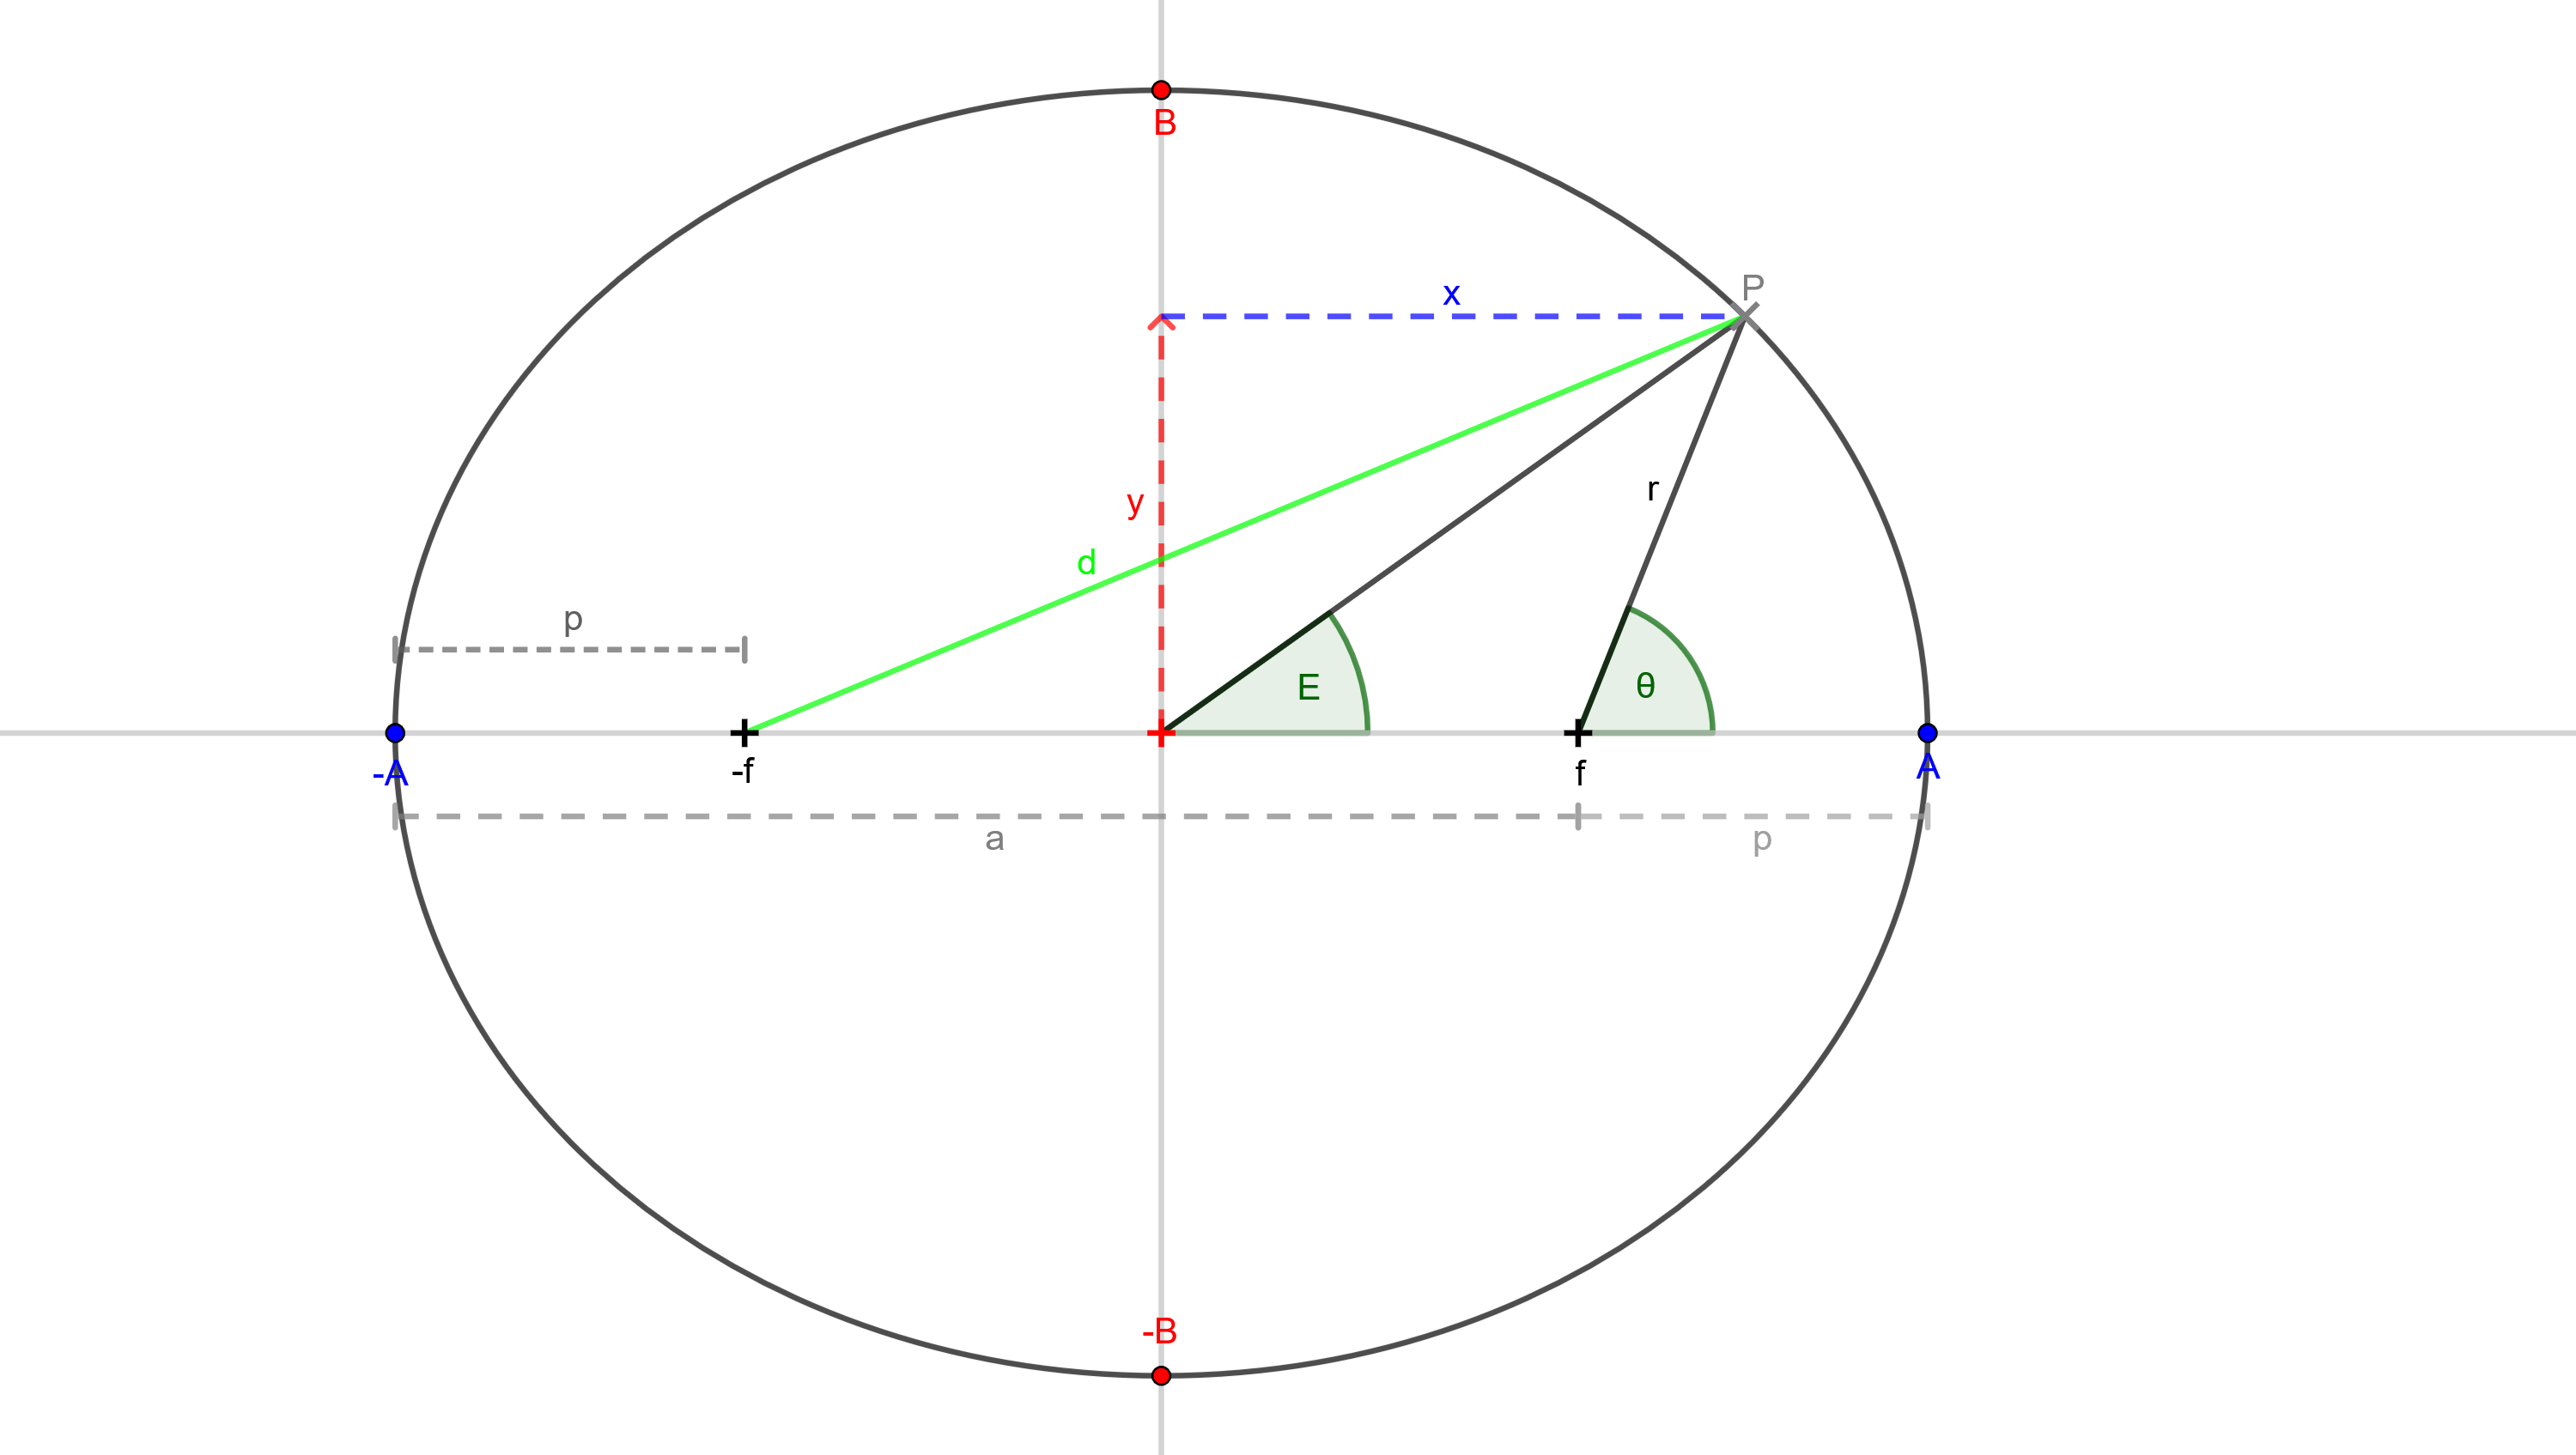
\includegraphics[width=0.8\textwidth]{./img/elipse.png} 
\caption{An Elipse with important values shown} \label{fig:GeometryElipse}
\end{figure}

In figure \ref{fig:GeometryElipse} a point $P$ on the ellipse forms an angle $E$ with the origin and the $x$ axis, this angle is called the \emph{Eccentric Anomaly}.

Also the angle $\theta$ is formed at the ellipse's focus between the point on the ellipse and the axis.

We also define the distances $a$ and $p$ as the apoapsis and periapsis distances respectively.

The semi major axis has been labeled as $A$, so that the total width of the ellipse is $2A$. Also shown on the diagram is the semi minor axis $B$, so the total height of the ellipse is $2B$.

For this text we will take the elliptical eccentricity to be defined as the ratio of the focus and the semi major axis.
\begin{equation}
e = \frac{f}{A} \label{eq:ecentricity}
\end{equation}
\subsection{The Apses}
Before we get any further, we will look at the apses. From figure \ref{fig:GeometryElipse} we can see that

\begin{equation}
p = A - f = A - eA = A(1-e)
\end{equation}

and that
\begin{equation}
a  = A + f = A + eA = A(1+e)
\end{equation}

also

\begin{align}
a+p &= A -f + A +f = 2A \\
a-p &= A + f - A + f = 2f
\end{align}

which can give us the eccentricity as defined by the apses
\begin{equation}
e=\frac{f}{A}=\frac{2f}{2A}=\frac{a-p}{a+p}
\end{equation}

\subsection{Sum of distances from foci and $P$}

One property of an ellipse is that the sum of the distances from any point on the ellipse and the foci is a constant. This fact allows you to draw an ellipse using two pins and a piece of string. We will use this fact and look at two special cases, before looking at the general case and deriving the equation for an ellipse. Before we do we will define what the sum is here.

\begin{equation}
S=d+r \label{eq:elipseConstraint}
\end{equation}

\paragraph{Special Case 1: Point on the $x$ axis}

When the point is at $(A,0)$. The distance $d$ is $f+A$ and the distance $r$ is $A-f$ from the diagram above. So our sum becomes

\begin{equation}
S = d + r = f+A + A-f = 2A \label{eq:ElipseSum}
\end{equation}

\paragraph{Special Case 2: Point on the $y$ axis}

When the point is on the $y$ axis, it is at the point $(0,B)$. The distance $d$ is $\sqrt{f^2+B^2}$ and the distance $r$ is also $\sqrt{f^2+B^2}$ from the diagram above. So our sum is

\begin{equation}
S = 2 \sqrt{f^2+B^2}
\end{equation}

and if the sum is a constant then this will be equal to the value obtained before\footnote{equation \ref{eq:ElipseSum}}.

\begin{equation}
S = 2 \sqrt{f^2+B^2} = 2 A
\end{equation}

and so we now have the relationship between the semi major and minor axes and the focus

\begin{equation}
 A^2=f^2+B^2
\end{equation}

This can also be used to get $B$ in terms of $A$ using the connection to the eccentricity\footnote{equation \ref{eq:ecentricity}}

\begin{align}
B^2&=A^2-f^2\nonumber \\
&=A^2-(eA)^2\nonumber \\
&=A^2(1-e^2)\nonumber \\
\Rightarrow  & B = A\sqrt{1-e^2}
\end{align}

\paragraph{General case}

In general for a point at $(x,y)$ we get the following
\begin{align}
r^2&=(x-f)^2+y^2\\
d^2&=(x+f)^2+y^2
\end{align}

by looking at the triangles formed in figure \ref{fig:GeometryElipse} with hypotenuse being $r$ and $d$ respectively. The sum\footnote{equation \ref{eq:elipseConstraint}} then becomes 

\begin{align}
S=2A&=\sqrt{(x-f)^2+y^2}+\sqrt{(x+f)^2+y^2}\nonumber \\
2A-\sqrt{(x-f)^2+y^2} &= \sqrt{(x+f)^2+y^2}
\end{align}

squaring both sides gives
\begin{align}
\left( 2A-\sqrt{(x-f)^2+y^2} \right)^2 &= (x+f)^2+y^2\nonumber \\
4A^2-4A\sqrt{(x-f)^2+y^2}+(x-f)^2+y^2  &= (x+f)^2+y^2\nonumber \\
4A^2-4A\sqrt{(x-f)^2+y^2}+x^2-2xf+f^2  &= x^2+2xf+f^2\nonumber \\
4A^2-4A\sqrt{(x-f)^2+y^2} &= 4xf\nonumber \\
4A^2-4xf &= 4A\sqrt{(x-f)^2+y^2}\nonumber \\
\frac{4A^2-4xf}{4A} &= \sqrt{(x-f)^2+y^2}\nonumber \\
\sqrt{(x-f)^2+y^2} &=A-\frac{xf}{A}
\end{align}

Squaring both sides gives again gives
\begin{align}
(x-f)^2+y^2 &=\left(A-\frac{xf}{A}\right)^2\nonumber \\
x^2-2xf+f^2+y^2 &=A^2-2\frac{xfA}{A}+\frac{x^2f^2}{A^2}\nonumber \\
x^2-2xf+f^2+y^2 &=A^2-2xf+e^2x^2\nonumber \\
(1-e^2)x^2+y^2 &=A^2-f^2\nonumber \\
(1-e^2)x^2+y^2 &=A^2(1-e^2)\nonumber \\
\frac{(1-e^2)x^2}{A^2(1-e^2)}+\frac{y^2}{A^2(1-e^2)}&=1\nonumber \\
\frac{x^2}{A^2}+\frac{y^2}{B^2}&=1 \label{eq:ElipseCartesian}
\end{align}

Which is the cartesian form of an elipse, there by showing that the elipse does indeed obey the contstraint that the sum of the distances from the foci is a constant.

\paragraph{Polar Form}

Once again returning to figure \ref{fig:GeometryElipse} we can see that 

\begin{align}
x &= f+r\cos \theta \\
y &= r \sin \theta
\end{align}

The sum\footnote{equation \ref{eq:elipseConstraint}} then becomes

\begin{align}
S = 2A &= r + d\nonumber \\
2A -r &= d
\end{align}

We can square both sides to get

\begin{align}
\left(2A -r\right)^2 &= d^2\nonumber \\
4A^2 -4Ar +r^2 &= (x+f)^2+y^2\nonumber \\
&= x^2+2fx+f^2+y^2\nonumber \\
&= \left(f+r \cos \theta\right)^2+2fx+f^2+r^2\sin^2\theta \nonumber \\
&= f^2+2fr \cos \theta + r^2 \cos^2\theta+2f\left(f+r \cos \theta\right)+f^2 \nonumber \\
&+r^2\sin^2\theta \nonumber \\
 &= f^2+2fr \cos \theta +2f^2+2fr \cos\theta+f^2\nonumber \\
&+r^2(\sin^2\theta+\cos^2\theta)\nonumber \\
 &= 4f^2+4fr \cos \theta+r^2\nonumber \\
A^2 -Ar &= f^2+fr \cos \theta\nonumber \\
A^2 -f^2 &= \left( A+f \cos \theta\right) r\nonumber \\
A^2 -e^2A^2 &= \left( A+eA \cos \theta\right) r\nonumber \\
A^2\left(1-e^2\right)&= A\left( 1+e \cos \theta\right) r\nonumber \\
A\left(1-e^2\right)&= \left( 1+e \cos \theta\right) r
\end{align}

Which with some rearranging results in the polar form for the equation of an elipse
\begin{equation}
r = \frac{A\left(1-e^2\right)}{ 1+e \cos \theta}
\end{equation}

\subsection{Relationship between $\theta$ and $E$}

Looking at figure \ref{fig:GeometryElipse} again we can see that $x$ and $y$ can also be given by

\begin{align}
x &= A \cos E \\
y &= B \sin E = A \sqrt{1-e^2} \sin E
\end{align}

We can also see that $r$ can be given by

\begin{align}
r^2 &= (x-f)^2 + y^2\nonumber \\
&= x^2-2xf+f^2 + y^2\nonumber  \\
&= A^2 \cos^2 E-2eA^2\cos E+e^2A^2 + A^2(1-e^2)\sin^2 E\nonumber  \\
\left(\frac{r}{A}\right)^2 &=  \cos^2 E-2e\cos E+e^2 + (1-e^2)\sin^2 E\nonumber  \\
\left(\frac{r}{A}\right)^2 &=  \cos^2 E-2e\cos E+e^2 + \sin^2 E-e^2\sin^2 E\nonumber  \\
\left(\frac{r}{A}\right)^2 &=  \left(\sin^2 E+\cos^2 E\right)-2e\cos E+e^2(1-\sin^2 E)\nonumber  \\
\left(\frac{r}{A}\right)^2 &=  1-2e\cos E+e^2\cos^2 E\nonumber  \\
\left(\frac{r}{A}\right)^2 &=  (1)^2-2(1)(e\cos E)+(e\cos E)^2\nonumber  \\
\left(\frac{r}{A}\right)^2 &=  \left( 1-e\cos E\right)^2
\end{align}

leading to
\begin{equation}
r = A\left( 1-e\cos E\right) \label{eq:radiusVsEccentric Anomaly}
\end{equation}
\clearpage

\section{Kepler's Equation}
%Derive Kepler's Equation to show time evolution in the perifocal plane
\section{Angular rates of change}
Starting with equation \refpage{eq:geom-radius} that gives the relationship between the distance from the focus and the ecentric anomaly
\begin{equation*}
r=A(1-e\cos E)
\end{equation*}
We can take the derivative with respect to time to get the relationship between the rate of change of distance with time and the ecentric anomally.
\begin{align}
\frac{dr}{dt} &= A \frac{d}{dt}\left(1-e\cos E \right)\nonumber \\
&= A \frac{dE}{dt}\frac{d}{dE}\left(1-e\cos E \right)\nonumber \\
&= eA \sin E \frac{dE}{dt} \label{eq:Kepler1}
\end{align}
Using equation \refpage{eq:geom-polar-form} for the equation of an elipse in polar form $r = \frac{A\left(1-e^2\right)}{ 1+e \cos \nu}$. We can invert this this to get

\begin{equation}
\frac{1}{r}= \frac{ 1+e \cos \nu}{A\left(1-e^2\right)} \\
\end{equation}
which will make taking the derivative with respect to time easier.
\begin{align}
\frac{d}{dt}\left( \frac{1}{r}\right) &= \frac{d}{dt}\left[ \frac{ 1+e \cos \nu}{A\left(1-e^2\right)}\right]\nonumber \\
\frac{dr}{dt}\frac{d}{dr}\left( \frac{1}{r}\right) &= \frac{1}{A(1-e^2)}\frac{d\nu}{dt}\frac{d}{d\nu}\left[  1+e \cos \nu \right]\nonumber \\
-\frac{1}{r^2}\frac{dr}{dt} &= \frac{-e \sin \nu}{A(1-e^2)}\frac{d\nu}{dt}
\end{align}
we can now substitute in equation \ref{eq:Kepler1} for $\frac{dr}{dt}$ to get
\begin{equation}
-\frac{1}{r^2} eA \sin E \frac{dE}{dt}= \frac{-e \sin \nu}{A(1-e^2)}\frac{d\nu}{dt} \label{eq:Kepler2}
\end{equation}
We can use equation \refpage{eq:geom-Xy} and \refpage{eq:geom-y} for y to obtain a relationship between $\sin \nu$ and $\sin E$
\begin{equation}
y = r \sin \nu = A\sqrt{1-e^2}\sin E
\end{equation}
We can use this relationship to replace the $\sin \nu$ term in equation \ref{eq:Kepler2}
\begin{align}
-\frac{1}{r^2} eA \sin E \frac{dE}{dt}&= \frac{-e \sin \nu}{A(1-e^2)}\frac{d\nu}{dt}\nonumber \\
&= \frac{-e A\sqrt{1-e^2}\sin E}{Ar(1-e^2)}\frac{d\nu}{dt}\nonumber \\
&= \frac{-e \sin E}{r\sqrt{1-e^2}}\frac{d\nu}{dt}\nonumber \\
\frac{-eA \sin E }{r^2} \frac{dE}{dt}&= \frac{-e \sin E}{r\sqrt{1-e^2}}\frac{d\nu}{dt}\nonumber \\
\frac{dE}{dt}&= \frac{-r^2}{eA \sin E } \frac{-e \sin E}{r\sqrt{1-e^2}}\frac{d\nu}{dt}\nonumber \\
\frac{dE}{dt} & = \frac{r}{A\sqrt{1-e^2}}\frac{d\nu}{dt}
\end{align}
Finally we can replace $r$ with equation \refpage{eq:geom-radius} $r=A(1-e \cos E)$ to get
\begin{align}
\frac{dE}{dt} & = \frac{r}{A\sqrt{1-e^2}}\frac{d\nu}{dt}\\
 & = \frac{A(1-e\cos E)}{A\sqrt{1-e^2}}\frac{d\nu}{dt}\\
  & = \frac{(1-e\cos E)}{\sqrt{1-e^2}}\frac{d\nu}{dt}\label{eq:Kepler3}
\end{align}
Now we have an equation that links the rate of change of $E$ to the rate of change of $\nu$ in terms of just $E$ and $\nu$

\section{Using Angular Momentum}

We can now use the magnitude of specific angular momentum in perifocal coordinates, given by equation \footnote{to review}
to replace $\dot{\nu}$
\begin{equation*}
\frac{d\nu}{dt} = \frac{h}{r^2}
\end{equation*}
useing equation \refpage{eq:geom-radius} and rearranging we obtain
\begin{align}
\frac{d\nu}{dt}&=\frac{h}{r^2}\nonumber \\
\frac{d\nu}{dt}&= \frac{h}{A^2\left(1-e \cos E \right)^2}
\end{align}
which we can now substitute in for $\frac{d\nu}{dt}$ term in equation \refpage{eq:Kepler3}
\begin{align}
\frac{dE}{dt} & = \frac{(1-e\cos E)}{\sqrt{1-e^2}}\frac{d\nu}{dt}\nonumber \\
& = \frac{(1-e\cos E)}{\sqrt{1-e^2}}\frac{h}{A^2\left(1-e \cos E \right)^2}\nonumber \\
&= \frac{h}{A^2\sqrt{1-e^2}}\frac{1}{1-e \cos E}\nonumber \\
\left(1-e \cos E \right)\frac{dE}{dt}&= \frac{h}{A^2\sqrt{1-e^2}}
\end{align}
Now you can see that the right hand side is just a constant, 
which is defined by properties of the orbit.
An interesting thing to note is that the term $A^2\sqrt{1-e^2}$ can be
rewritten as the product $AB$ instead, so linking the major and minor axes.
We will however keep it in it's original form for now. Since the right hand
side is a constant we will simplify by choosing the constant $n$ for it. 
This constant $n$ is the \emph{Mean Motion}, later we will see that it's 
connected to the period of the orbit, and ends up being the mean 
angular velocity of the orbiting body.
\begin{equation}
n = \frac{\frac{l}{m}}{A^2\sqrt{1-e^2}}\label{eq:Kepler4}
\end{equation}
so finally all that is left to do is to integrate our equation with respect to time.
\begin{align}
\int_{t_0}^t n dt &= \int_{t=t_0}^t\left(1-e \cos E \right)\frac{dE}{dt} dt\nonumber \\
n (t-t_0) &=\int_{E=0}^E\left(1-e \cos E \right)dE \nonumber \\
&=\int_0^E 1 dE - e \int_0^E \cos E dE\nonumber \\
&=E - e \sin E\\
\end{align}
Note we have chosen $t_0$ to be the point in time when $E=0$, or in words
the time since periapsis at epoch.
\begin{equation}
E - e \sin E=n(t-t_0)
\end{equation}
If we define the \emph{Mean Anomally} to be $M = n(t-\tau)$,
where we have given $t_0$ a new label $\tau = t_0$, because it is a parameter
that determines something about the orbit.

We can now rewrite the equation in the more standard form of 
\begin{equation}
E - e \sin E=M
\end{equation}
With $M$ being
\begin{equation}
M = n(t-\tau) = nt - M_0
\end{equation}
where $M_0$ is the mean anomally at epoch, and is just another way to state $\tau$.
It is the angle the orbiting body would be at if the orbit was circular from the periapsis
at time zero.

\section{Mean Motion}

We previously stated that the mean motion was related to the period without actually showing it.
Here we will show the relationship. Because of the way we have integrated, we have chosen to make
$\tau$ the time when the eccentric anomally $E$ is zero, this means that at $t=0$ the eccentric
anomally is
\begin{align}
M(t=0)&= -n\tau \nonumber \\
E_0 - e \sin E_0 & = -n\tau
\end{align}

When the orbiting body has gone through a whole orbit, the time 
taken to do that will be $T$, or the period. The eccentric anomally will then be $E=2\pi+E_0$, because
it has completed a full circle in terms of angle around the centre of the ellipse. So the mean
anomally is

\begin{align}
M(t=T)&= nT - n\tau \nonumber \\
nT - n\tau&=2\pi +E_0 - e \sin (2\pi + E_0)\nonumber \\
&=2\pi +E_0 - e \sin (E_0)\nonumber \\
&= 2\pi -n\tau\nonumber \\
nT &= 2\pi \nonumber \\
n &= \frac{2\pi}{T}
\end{align}

\clearpage

\section{Eliptical Orbits}
\subsection{Elipse}

\begin{figure}[h]
\centering
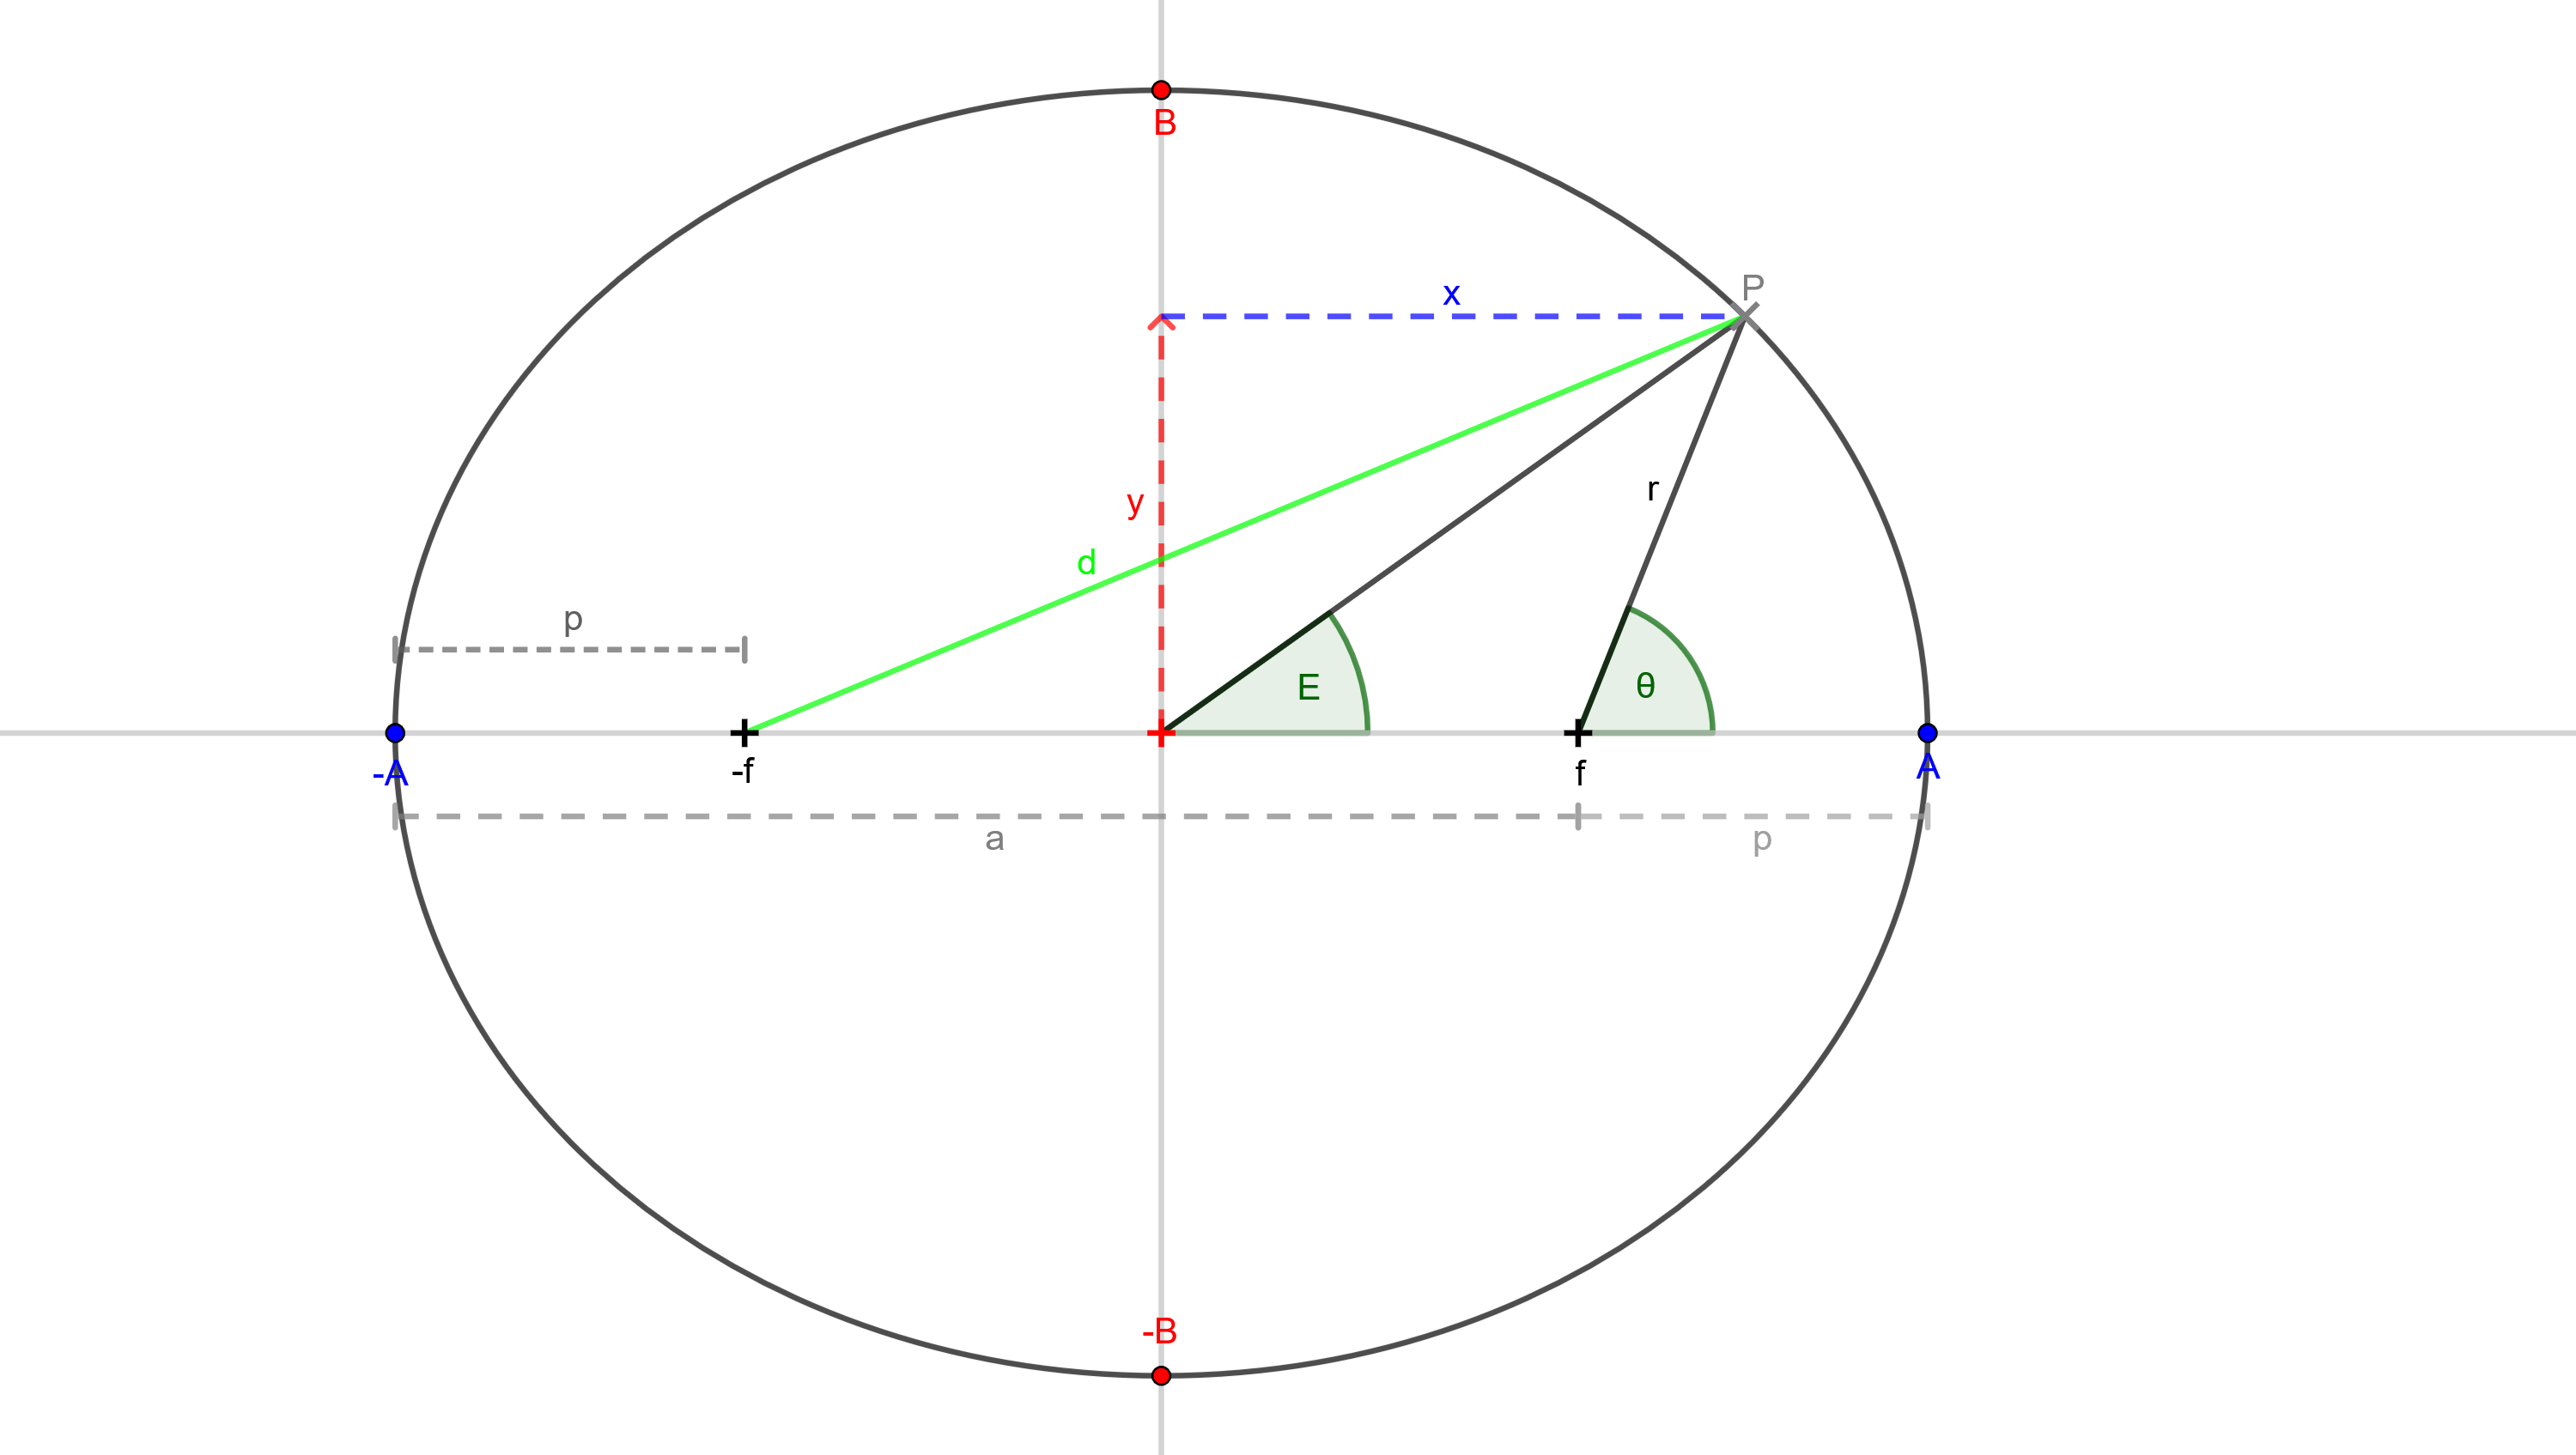
\includegraphics[width=0.8\textwidth]{./img/elipse.png} 
\caption{An Elipse with important values shown} \label{fig:GeometryElipse}
\end{figure}

In the above diagram a point $P$ on the ellipse forms an angle $E$ with the origin and the $x$ axis. Also the angle $\theta$ is formed at the ellipse's focus between the point on the ellipse and the axis.

We also define the distances $a$ and $p$ as the apoapsis and periapsis distances respectively.

The semi major axis has been labeled as $A$, so that the total width of the ellipse is $2A$. Also shown on the diagram is the semi minor axis $B$, so the total height of the ellipse is $2B$.

For this text we will take the elliptical eccentricity to be defined as the ratio of the focus and the semi major axis.
\begin{equation}
e = \frac{f}{A}
\end{equation}
\subsubsection{The Apses}
Before we get any further, we will look at the apses. From figure \ref{fig:GeometryElipse} we can see that

\begin{equation}
p = A - f = A - eA = A(1-e)
\end{equation}

and that
\begin{equation}
a  = A + f = A + eA = A(1+e)
\end{equation}

also

\begin{align}
a+p &= A -f + A +f = 2A \\
a-p &= A + f - A + f = 2f
\end{align}

which can give us the eccentricity as defined by the apses
\begin{equation}
e=\frac{f}{A}=\frac{2f}{2A}=\frac{a-p}{a+p}
\end{equation}

\subsubsection{Sum of distances from foci and $P$}

One property of an ellipse is that the sum of the distances from any point on the ellipse and the foci is a constant. This fact allows you to draw an ellipse using two pins and a piece of string. We will use this fact and look at two special cases, before looking at the general case and deriving the equation for an ellipse. Before we do we will define what the sum is here.

\begin{equation}
S=d+r
\end{equation}

\paragraph{Special Case 1: Point on the $x$ axis}

When the point is at $(A,0)$. The distance $d$ is $f+A$ and the distance $r$ is $A-f$ from the diagram above. So our sum becomes

\begin{equation}
S = d + r = f+A + A-f = 2A
\end{equation}

\paragraph{Special Case 2: Point on the $y$ axis}



\subsection{Solving equtaions of motion}

Firstly we let $r=\frac{1}{u}$, so that

\begin{align}
\frac{dr}{dt} &= \frac{du^{-1}}{dt}\nonumber \\
&= \frac{du^{-1}}{du}\frac{du}{dt}\nonumber \\
&= -\frac{1}{u^2}\frac{du}{dt}\nonumber \\
&= -r^2\frac{du}{dt}
\end{align}

next we introduce an $\omega$ by chain rule

\begin{align}
\frac{dr}{dt}
&= -r^2\frac{du}{dt}\nonumber \\
\frac{dr}{dt} &= -r^2\frac{du}{d\theta}\frac{d\theta}{dt} \nonumber \\
&= -r^2\omega\frac{du}{d\theta} \nonumber
\end{align}

And using the magnitude of angular momentum\footnote{equation \ref{eq:AngularMomentumScalar}} $l=mr^2\omega$ or rearranging $\omega = \frac{l}{mr^2}$

\begin{align}
\frac{dr}{dt}&= -r^2\omega\frac{du}{d\theta} \nonumber \\
\frac{dr}{dt}&= -r^2\frac{l}{mr^2}\frac{du}{d\theta} \nonumber \\
\frac{dr}{dt}&= -\frac{l}{m}\frac{du}{d\theta} \nonumber \\
\frac{dr}{dt}&= -\frac{l}{m}\frac{du}{d\theta}
\end{align}

Differentiating again with respect to time gives

\begin{align}
\frac{dr^2}{dt^2}&= -\frac{l}{m}\frac{d}{dt}\frac{du}{d\theta} \nonumber \\
&= -\frac{l}{m}\frac{d\theta}{dt}\frac{d}{d\theta}\frac{du}{d\theta}\nonumber \\
&= -\frac{l}{m}\omega\frac{d^2u}{d\theta^2}
\end{align}

We can substitute the magnitude of angular momentum\footnote{equation \ref{eq:AngularMomentumScalar}} $l=mr^2\omega$ again to get

\begin{align}
\frac{dr^2}{dt^2}&= -\frac{l}{m}\omega\frac{d^2u}{d\theta^2} \nonumber \\
&= -\frac{mr^2\omega}{m}\omega\frac{d^2u}{d\theta^2} \nonumber \\
&= -r^2\omega^2\frac{d^2u}{d\theta^2}
\end{align}

We can now substitute this into the radial part of the acceleration\footnote{equation \ref{eq:radialAcceleration}}

\begin{align}
-\frac{GM}{r^2}&= \frac{ d^2 r}{d t^2} -r \omega^2  \nonumber \\
&=-r^2\omega^2\frac{d^2u}{d\theta^2} -r\omega^2 \nonumber \\
&=-r^2\omega^2\left[\frac{d^2u}{d\theta^2}+\frac{1}{r}\right] \nonumber \\
GM&=r^4\omega^2\left[\frac{d^2u}{d\theta^2}+\frac{1}{r}\right]
\end{align}

Next we recall that $u=\frac{1}{r}$ and that $\frac{l}{m}=r^2\omega$ and substitute these in

\begin{align}
GM&=\left(\frac{l}{m}\right)^2\left[\frac{d^2u}{d\theta^2}+u\right] \nonumber\\
\frac{d^2u}{d\theta^2}+u &=\frac{GMm^2}{l^2}
\end{align}

To simplify this equation we will use $\alpha=\frac{GMm^2}{l^2}$

\subsubsection{Solution}

The direct solution to
\begin{equation}
\frac{d^2u}{d\theta^2}+u =\alpha
\end{equation}

is $u=\alpha$

However because there is also a function that results in zero, we must include that

\begin{align}
\frac{d^2u}{d\theta^2}+u &=0 \nonumber \\
\frac{d^2u}{d\theta^2} &=-u
\end{align}

we can take the solution that $u=c\cos\theta$ which gives the general overall solution of

\begin{equation}
u(\theta)=\alpha + c \cos \theta
\end{equation}

We can pick an initial condition when $\theta=0$ the body is at periapsis or $r=p=A(1-e)$ which gives $u=\frac{1}{A(1-e)}$ (see the ellipse notes for $p=A(1-e)$)


\begin{align}
\frac{1}{A(1-e)}&=\alpha+c \nonumber \\
\alpha&=\frac{1}{A(1-e)} - c
\end{align}


we could similarly hae picked the condition that when $\theta=\pi$ the body is at apoapsis or $r=a=A(1+e)$ which gives $u=\frac{1}{A(1+e)}$ (see ellipse notes for $a=A(1+e)$)


\begin{align}
\frac{1}{A(1+e)}&=\alpha-c \nonumber \\
\alpha&=\frac{1}{A(1+e)} + c
\end{align}

we can equate our two initial conditions to get $c$ in terms of just $a$ and $p$

\begin{align}
\alpha=\frac{1}{A(1-e)}-c&=\frac{1}{A(1+e)} + c \nonumber \\
\frac{1}{A(1-e)}-\frac{1}{A(1+e)}&=2c \nonumber \\
\frac{A(1+e)-A(1-e)}{A^2(1+e)(1-e)}&=2c \nonumber \\
\frac{A+eA-A+eA}{A^2(1-e^2)}&=2c \nonumber \\
\frac{2eA}{A^2(1-e^2)}&=2c \nonumber \\
\frac{e}{A(1-e^2)}&=c
\end{align}

Now that we have $c$ we can use this to determine $\alpha$ in terms of $A$ and $e$

\begin{align}
\alpha&=\frac{1}{A(1+e)} + c \nonumber \\
&=\frac{1}{A(1+e)} + \frac{e}{A(1-e)^2}\nonumber \\
&=\frac{(1-e)}{A(1+e)(1-e)} + \frac{e}{A(1-e)^2}\nonumber \\
&=\frac{1-e+e}{A(1-e^2)} \nonumber \\
&=\frac{1}{A(1-e^2)} \nonumber
\end{align}

So feeding all this back in we have

\begin{align}
u(\theta)&=\alpha + c \cos \theta \nonumber \\
&=\frac{1}{A(1-e^2)} + \frac{e}{A(1-e^2)} \cos \theta \nonumber \\
&=\frac{1+e\cos\theta}{A(1-e^2)}
\end{align}

Now we have a simple form for $u$ we can recall that we chose $u=\frac{1}{r}$, so

\begin{equation}
r=\frac{1+e\cos\theta}{A(1-e^2)}
\end{equation}

which is the equation for a ellipse we saw from the ellipse notes.

We also get the interesting result here that

\begin{align}
\alpha = \frac{GMm^2}{l^2}&=\frac{1}{A(1-e^2)} \nonumber \\
A(1-e^2)&=\frac{l^2}{GMm^2}
\end{align}

\clearpage

\section{Relationship between geometry and physics}
We saw in the previous chapter that the geometry and the physics were linked by equation \ref{eq:link}.

\subsection{Angular Momentum From Geometry}

We can rearrange equation \ref{eq:link} to get

\begin{align}
\frac{l^2}{GMm^2} &= A(1-e^2)\nonumber \\
&=\frac{A^2(1-e^2)}{A} \nonumber \\
&=\frac{B^2}{A} \nonumber \\
&=\frac{ap}{A} \nonumber \\
&=\frac{2ap}{a+p}
\end{align}

With some further rearrangement we can obtain the angular momentum per unit mass of the orbiting body

\begin{align}
\frac{l^2}{GMm^2} &=\frac{2ap}{a+p} \nonumber \\
\left(\frac{l}{m}\right)^2 &= GM \frac{2ap}{a+p} \nonumber \\
\frac{l}{m}&=\sqrt{GM  \frac{2ap}{a+p}}
\end{align}

\subsection{Total Energy From Geometry}


\clearpage

\section{In Plane Position and Velocity over time}
We will assume that the apses are know as well as the central mass. From this the period is given by equation~\ref{eq:PeriodApses} on page~\pageref{eq:PeriodApses}
\begin{equation*}
T =\sqrt{ \frac{4 \pi^2 }{GM}}\left(\frac{a+p}{2}\right)^\frac{3}{2}
\end{equation*}
At any given time we can calculate the ecentric anomaly $E$ using Kepler's Equation\footnote{equation~\ref{eq:KeplersEquation2} on page~\pageref{eq:KeplersEquation2}}
\begin{equation*}
E-e\sin E = 2\pi\frac{(t-t_0)}{T}
\end{equation*}
Since this is trancendental, it will need to be solved numerically, or by approximation. This text will not cover those methods, and assume that $E$ can be determined as a function of $t$.

\subsection{Position}
Once $E$ is known, then the position can de determined by
\begin{align*}
e&=\frac{a-p}{a+p}\\
r&=A\left( 1-e\cos E\right)\\
x&=r\cos\theta =A(\cos(E)-e)\\
y&=r\sin\theta = A\sqrt{1-e^2}\sin E
\end{align*}

\subsection{Velocitiy}

\subsubsection{Angular Velocity}

Using equation~\ref{eq:Connection1} on page~\pageref{eq:Connection1} to get the angular momentum
\begin{equation*}
\left(\frac{l}{m} \right) =\sqrt{GM}\sqrt{\frac{2ap}{a+p}}
\end{equation*}
and using equation~\ref{} on page~\pageref{}, we can get the angular velocity as
\begin{equation}
\omega = \frac{l}{m}\frac{1}{r^2}=\sqrt{GM}\sqrt{\frac{2ap}{a+p}}\frac{1}{r^2}
\end{equation}

\subsubsection{Radial velocity}
The radial velocity we obtain from the geometry. Recall that we have
\begin{equation}
r=A(1-e\cos E)
\end{equation}
As we did for the derivation of Kepler's Equation, we can differentiate with respect to time. Which gives the result
\begin{equation}
\frac{dr}{dt} =eA \sin E \frac{dE}{dt}
\end{equation}
And looking at Kepler's Equation again
\begin{align*}
E-e\sin E &= 2\pi\frac{t-t_0}{T}\\
t&=\frac{E-e\sin E}{2\pi}T+t_0\\
\frac{dt}{dE}&=\frac{1-e\cos E}{2\pi}T
\end{align*}
which gives us the result that
\begin{equation}
\frac{dE}{dt}=\frac{2\pi}{T}\frac{1}{1-e\cos E}
\end{equation}
We can put this back in to our earlier equation to get the radial velocity
\begin{equation}
\frac{dr}{dt} = \frac{2\pi}{T}\frac{ eA \sin E}{1-e\cos E}
\end{equation}

\clearpage

%\section{Solving equations of motion}
%\input{./tex/Solution.tex}
%\clearpage

%\section{Apoapsis and Periapsis}
%\input{./tex/ApoPeri.tex}
%\clearpage

%\section{Circular Orbits}
%\input{./tex/Circular.tex}
%\clearpage

%\section{Elliptical Orbits}
%\input{./tex/Eliptical.tex}
%\clearpage

\end{document}